\documentclass[conference]{IEEEtran}

\usepackage{graphicx}
\usepackage{amsmath}
\usepackage{listings}
\usepackage{color}
\usepackage{url}
\usepackage{hyperref}
\usepackage{cite}
\usepackage[utf8]{inputenc}
\usepackage{courier}
\usepackage{tabularx} % For adjustable width tables
\usepackage{booktabs} % For better table formatting
\usepackage{array}    % For additional column formatting
\usepackage{ragged2e} % For better text justification
\usepackage{float} % Add to preamble


\usepackage{fancyhdr}
\pagestyle{fancy}
\fancyhf{}
\cfoot{\thepage}
\renewcommand{\headrulewidth}{0pt}


% Code listing style
\definecolor{codegreen}{rgb}{0,0.6,0}
\definecolor{codegray}{rgb}{0.5,0.5,0.5}
\definecolor{backcolour}{rgb}{0.95,0.95,0.92}

\hypersetup{
    colorlinks=true,    % false: boxed links; true: colored links
    linkcolor=black,    % color of internal links
    citecolor=black,    % color of citation links
    urlcolor=black      % color of external web links
}



\lstdefinestyle{style}{
    backgroundcolor=\color{backcolour},   
    commentstyle=\color{codegreen},
    keywordstyle=\color{blue},
    numberstyle=\tiny\color{codegray},
    stringstyle=\color{codegreen},
    basicstyle=\fontfamily{pcr}\selectfont\footnotesize,
    breakatwhitespace=false,         
    breaklines=true,                 
    captionpos=b,                    
    keepspaces=true,                 
    numbers=left,                    
    numbersep=5pt,                  
    showspaces=false,                
    showstringspaces=false,
    showtabs=false,                  
    tabsize=2
}
\lstset{style=style}

\begin{document}


\title{
  \raisebox{-0.5\height}{
\includegraphics[height=1.5cm]{figs/iitjammu.png}}
  \hfill
  \parbox{0.8\textwidth}{\centering GEM5 Extensions: Broadening Support to Microcontrollers with GUI}
  \hfill
  \raisebox{-0.5\height}{
\includegraphics[height=1.5cm]{figs/gem5.png}}
}

\author{Ashutosh Vishwakarma (2022UCS0083)\\
	Guide: Dr. Subhasis Bhattacharjee\\
	\textit{Computer Science \& Engineering,
	Indian Institute of Technology, Jammu}}


\maketitle

\newpage

\begin{abstract}
	This is the introduction section. It describes the background and motivation for the research.
\end{abstract}

\section{Introduction}
In current state, different ISAs are available for systems, some favoured over others. Nonetheless,
three major ISAs are \texttt{ARM}, \texttt{RISCV} and \texttt{x86}. Each of them were designed in different
time period for different needs. Despite their differences these architectures are slowly being used in 
comparable machines with most computers still powered with Intel/AMDs \texttt{x86} and Macs \texttt{ARM}.
\texttt{RISCV} is gaining space as Linux based OS's like FreeBSD extending to support it. In this study we
aim to compare these ISAs on a common benchmark. We'll mostly focus on execution speed with and without 
caches. We'll be using the \texttt{gem5} simulation system for the same. \texttt{gem5} provides a 
huge suite of tools to test the CPU performance. Although we won't be getting into the \texttt{C++} core
of \texttt{gem5}, but we'll be using the \texttt{Python} api of \texttt{gem5} with the existing modules. 

\section{Literature Review}
The evolution of architectural simulators and their applications in computer architecture research has been extensively documented in the literature. This review synthesizes key findings across simulator development, architectural comparisons, and performance analysis methodologies.

\subsection{Architectural Simulation Frameworks}

The foundation of modern architectural simulation was established with the introduction of the gem5 simulator by Binkert et al.~\cite{binkert2011gem5}, which provided a flexible and extensible platform for computer architecture research. This framework has been continuously enhanced, as demonstrated by Power et al.~\cite{power2015gem5gpu} through their gem5-gpu extension, enabling heterogeneous CPU-GPU simulation capabilities.

The accuracy of architectural simulators has been rigorously evaluated, with Butko et al.~\cite{butko2012accuracy} providing comprehensive validation of the GEM5 simulator system. Recent developments include Lee et al.'s~\cite{lee2024gem5} extension of GEM5 to support AVX instruction sets, demonstrating the simulator's adaptability to new architectural features.

Alternative simulation frameworks have also emerged, including:
\begin{enumerate}
    \item ZSim by Sanchez and Kozyrakis~\cite{sanchez2013zsim}, focusing on thousand-core system simulation
    \item PTLsim by Yourst~\cite{yourst2007ptlsim}, offering cycle-accurate x86-64 simulation
    \item Sniper by Carlson et al.~\cite{carlson2011sniper}, exploring scalable multi-core simulation
    \item UNISIM by August et al.~\cite{august2007unisim}, providing an open environment for collaborative development
\end{enumerate}

\subsection{ISA Performance Analysis}

Comparative analysis of different instruction set architectures has been a crucial area of research. Bharadwaj and Vudadha~\cite{bharadwaj2022evaluation} conducted detailed evaluations of x86 and ARM architectures using compute-intensive workloads. This work was complemented by Ling et al.~\cite{ling2019isa}, who investigated the fundamental question of ISA impact on system performance.

The classical RISC versus CISC debate, initially explored by George~\cite{george1990overview} and later elaborated by Jamil~\cite{jamil1995risc}, continues to influence modern architectural decisions. Abudaqa et al.~\cite{abudaqa2018simulation} extended this comparison through detailed simulation studies of ARM and x86 processors using both in-order and out-of-order CPU models.

\subsection{Cache and Memory Performance}

Memory system optimization remains a critical aspect of architectural design:

\begin{enumerate}
    \item Saha et al.~\cite{saha2020impact} analyzed the impact of cache size and latency on system performance, providing crucial insights for memory hierarchy design
    \item Vikas and Talawar~\cite{vikas2014cache} studied cache behavior using Splash-2 benchmarks on ARM and Alpha processors, demonstrating the importance of cache optimization across different architectures
\end{enumerate}

\subsection{Research Gaps and Opportunities}

The literature review reveals several key areas requiring further investigation:

\begin{enumerate}
    \item Limited support for microcontroller architectures in mainstream simulators
    \item Need for comprehensive GUI-based debugging tools for architectural simulation
    \item Lack of standardized performance metrics for microcontroller simulation
    \item Gap in comparative studies involving emerging embedded architectures
\end{enumerate}

\subsection{Synthesis and Research Direction}

This review demonstrates the maturity of architectural simulation tools while highlighting the need for expanded support for microcontroller architectures. Our work builds upon these foundations, particularly extending GEM5's capabilities to support AVR architecture, addressing a significant gap in current simulation frameworks. The integration of GUI-based debugging tools and comprehensive performance analysis capabilities represents a natural evolution in architectural simulation technology.

\section{Methodology}
In this project, we proceeded in two phases. First, we explored Gem5's capabilities and developed a deeper understanding of the simulator's internal workings. To do this, we studied the impact of different instruction set architectures (ISAs) on execution speed and cache miss rates under a given workload. We used the Gem5 simulator to run a set of benchmarks and collected data on execution time and cache performance. This data was then analyzed to evaluate how different ISAs influence performance. The insights gained helped us identify the strengths and limitations of each ISA in various scenarios.

In the second phase, we worked on extending Gem5 to support the AVR architecture. We began by familiarizing ourselves with the existing codebase and identifying the components that required modification. We then implemented support for basic AVR instructions such as \texttt{add} and \texttt{sub}.

\subsection{Testing the gem5 simulator}
For the testing we used the algorithm of multiplying two matrices in row major format. The algorithm was written in C and compiled for different architectures.

\subsubsection{\textbf{Workload Compilation}} The used code was:
\begin{lstlisting}[language=C, caption={Row major matrix multiplication algorithm}, label={lst:matrix_mult}]
// Multiplication of two matrices
#include <stdio.h>
#include <stdlib.h>
#include <time.h>

int** createRandomMatrix(int n) {
    int** matrix = malloc(n * sizeof(int*));
    for (int i = 0; i < n; i++) {
        matrix[i] = malloc(n * sizeof(int));
        for (int j = 0; j < n; j++) {
            matrix[i][j] = (rand()%2==1?-1:1)*rand() % MAX; // capping the values
        }
    }
    return matrix;
}

int** createZeroMatrix(int n) {
    int** matrix = malloc(n * sizeof(int*));
    for (int i = 0; i < n; i++) {
        matrix[i] = calloc(n, sizeof(int));
    }
    return matrix;
}

void printMatrix(int** matrix, int n) {
    for (int i = 0; i < n; i++) {
        for (int j = 0; j < n; j++) {
            printf("%3d ", matrix[i][j]);
        }
        printf("\n");
    }
}

void multiplyMatrices(int** A, int** B, int** C, int n) {
    for (int i = 0; i < n; i++) {           // Row of A
        for (int j = 0; j < n; j++) {       // Column of B
            for (int k = 0; k < n; k++) {   // Iterate over row-col
                C[i][j] += A[i][k] * B[k][j];
            }
        }
    }
}

void freeMatrix(int** matrix, int n) {
    for (int i = 0; i < n; i++)
        free(matrix[i]);
    free(matrix);
}

int main() {
    int n = DIM;
    srand(time(NULL)); 

    int** A = createRandomMatrix(n);
    int** B = createRandomMatrix(n);
    int** C = createZeroMatrix(n);

    printf("Matrix A:\n");
    printMatrix(A, n);

    printf("\nMatrix B:\n");
    printMatrix(B, n);

    multiplyMatrices(A, B, C, n);

    printf("\nMatrix A x B:\n");
    printMatrix(C, n);

    freeMatrix(A, n);
    freeMatrix(B, n);
    freeMatrix(C, n);

    return 0;
}

\end{lstlisting}

The used code was compiled with two constants \texttt{DIM} and \texttt{MAX}. The constant \texttt{DIM} is the size of the matrix and the constant \texttt{MAX} is the maximum absolute value of the elements in the matrix. The code was compiled with the following command:

\begin{lstlisting}[language=bash , caption={Compilation Command}, label={lst:compilation}]
    <compiler> -static -o matrix_mult matrix_mult.c -DDIM=<dimension> -DMAX=<max_value>
\end{lstlisting}


The code was compiled with the \texttt{-static} flag to ensure that the code is statically linked. This is important because the gem5 simulator does not support dynamic linking. The code was compiled with the \texttt{-D} flag to define the constants \texttt{DIM} and \texttt{MAX}.

The code generates two random matrices of size \texttt{DIM} and multiplies them. The result is printed to the standard output. The code was compiled for the following architectures:

\begin{table}[h!]
	\centering
	\begin{tabular}{|c|c|c|}
		\hline
		\textbf{Architecture} & \textbf{Compiler}     \\
		\hline
		x86                   & gcc                   \\
		ARM                   & aarch64-linux-gnu-gcc \\
		RISCV                 & riscv-linux-gnu-gcc   \\
		\hline
	\end{tabular}
	\vspace{0.2cm}
	\caption{List of architectures and their compilers}
\end{table}

\subsubsection{\textbf{Simulation System Design}} The gem5 simulation has a modular design. It closely resembles a real system. The main part on which simulation run is a board. There are multiple types of boards in gem5. A board holds different components of a system namely clock, processor and memory. The binary resource is also loaded to this board.

\begin{lstlisting}[language=python, caption={Creating System Configuration for GEM5 simulation}, label={lst:gem5_processor}]
processor = SimpleProcessor(
    cpu_type=CPUTypes.TIMING,
    num_cores=1,
    isa=isa
)

memory = SingleChannelDDR3_1600("1GiB")

'''
Cache hierarchy can be defined in multiple ways.
For example, you can use a NoCache or a PrivateL1PrivateL2CacheHierarchy.
'''
cache_hierarchy = NoCache()

# or

cache_hierarchy = PrivateL1PrivateL2CacheHierarchy(
    l1d_size="32kB",
    l1i_size="32kB",
    l2_size="128kB"
)

board = SimpleBoard(
    clk_freq="1GHz",
    processor=processor,
    memory=memory,
    cache_hierarchy=cache_hierarchy
)

binary = BinaryResource("<path_to_binary>")
board.set_se_binary_workload(binary)

simulator = Simulator(board=board)
simulator.run()
\end{lstlisting}

The code in the listing \ref{lst:gem5_processor} shows how to create a system configuration for gem5 simulation. The code creates a simple board with a single core processor, memory and cache hierarchy. The binary resource is loaded to the board. The simulator is then run.
The code is written in Python. The gem5 simulator provides a Python API to create the system configuration. The code can be run with the following command:
\begin{lstlisting}[language=bash, caption={Running the simulation}, label={lst:gem5_run}]
./build/ALL/gem5.opt <path_to_script>
\end{lstlisting}
The code can be run with the \texttt{gem5.opt} binary. The \texttt{gem5.opt} binary is the optimized version of the gem5 simulator. The \texttt{gem5.debug} binary is the debug version of the gem5 simulator.

The simulation produces the results in \texttt{m5out} directory. The directory contains system configuration diagram and statistics.
\begin{figure}[h]
	\centering
	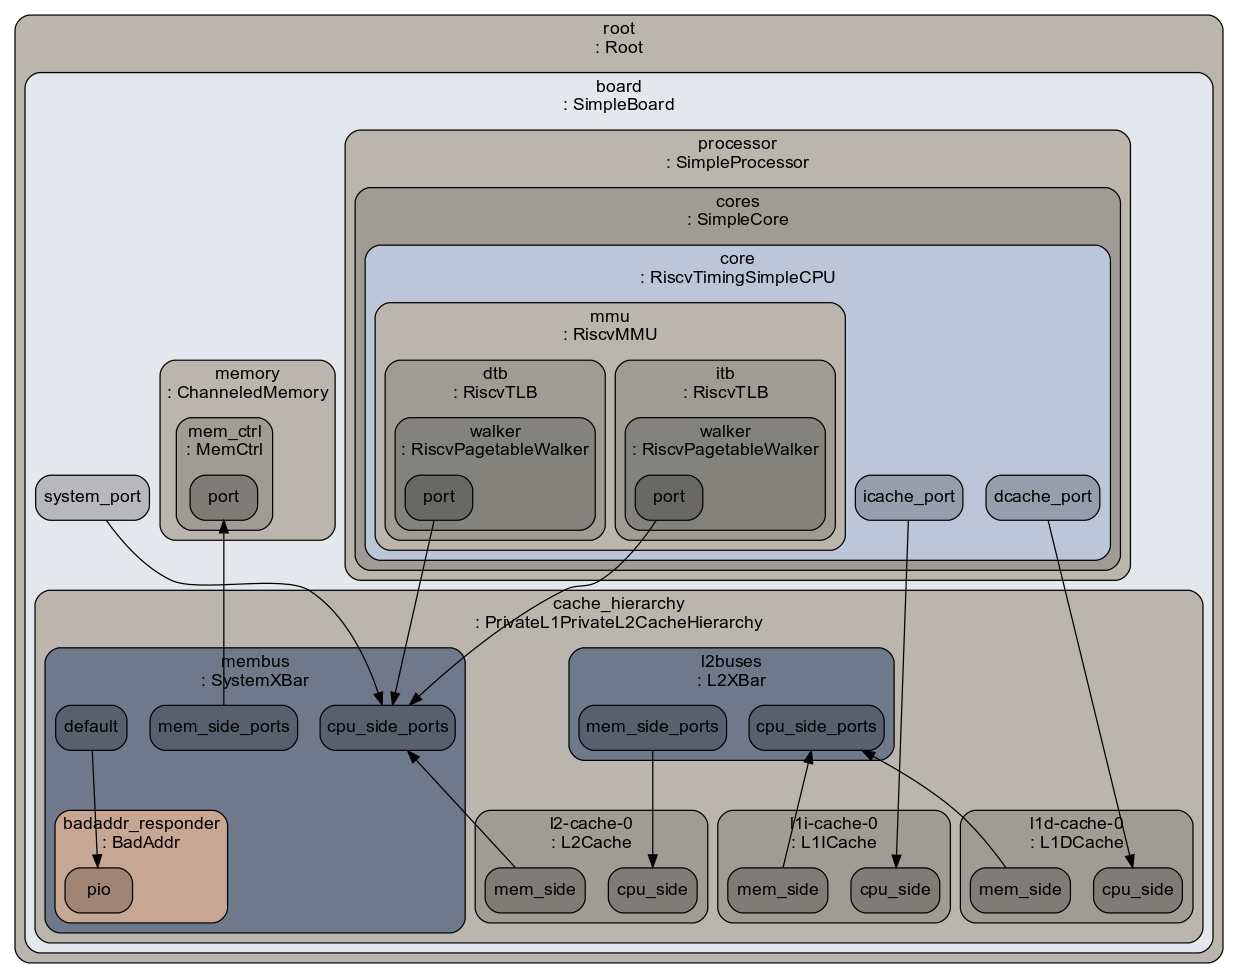
\includegraphics[width=8.5cm]{figs/config.dot.png}
	\caption{Sample System Configuration Diagram}
	\label{fig:system_config}
\end{figure}
The results are written to \texttt{stats.txt} file.

\begin{lstlisting}[language=python, caption={Sample Statistics}, label={lst:gem5_stats}]

---------- Begin Simulation Statistics ----------
simSeconds                                   0.000282                       # Number of seconds simulated (Second)
simTicks                                    281722000                       # Number of ticks simulated (Tick)
finalTick                                   281722000                       # Number of ticks from beginning of simulation (restored from checkpoints and never reset) (Tick)
simFreq                                  1000000000000                       # The number of ticks per simulated second ((Tick/Second))
hostSeconds                                      0.19                       # Real time elapsed on the host (Second)
hostTickRate                               1498170641                       # The number of ticks simulated per host second (ticks/s) ((Tick/Second))
hostMemory                                    4448164                       # Number of bytes of host memory used (Byte)
simInsts                                       172171                       # Number of instructions simulated (Count)
simOps                                         192213                       # Number of ops (including micro ops) simulated (Count)
hostInstRate                                   915165                       # Simulator instruction rate (inst/s) ((Count/Second))
                            ...
\end{lstlisting}

\subsubsection{\textbf{Simulation Parameters}} For the study of the gem5's simulation system,  we used following input parameters:
\begin{table}[ht]
	\centering
	\renewcommand{\arraystretch}{1.5} % Adjust for better vertical spacing
	\begin{tabularx}{7cm}{|>{\centering\arraybackslash}m{1.5cm}|>{\centering\arraybackslash}m{1.5cm}|>{\centering\arraybackslash}m{2.7cm}|}
		\hline
		\textbf{Parameters} & \textbf{Values}        & \textbf{Description}                                     \\
		\hline
		Architecture        & ARM, RISC-V, x86       & Instruction Set Architecture type used in the simulation \\
		\hline
		Cache Availability  & Yes, No                & Whether cache memory is available in the simulation      \\
		\hline
		L1D Size            & 32, 64, 128 kB         & Size of Level 1 data cache                               \\
		\hline
		L1I Size            & 32, 64, 128 kB         & Size of Level 1 instruction cache                        \\
		\hline
		L2 Size             & 128, 256, 512, 1024 kB & Size of Level 2 cache                                    \\
		\hline
		Matrix Dimension    & 5, 10, 20, 40, 80      & Dimension of the square matrix for multiplication        \\
		\hline
		max_val             & $10^6$                 & Maximum absolute value of the elements in the matrix     \\
		\hline
	\end{tabularx}
	\vspace{0.2cm}
	\caption{Parameters of Simulation}
	\label{tab:sim_params}
\end{table}

We restricted our study to execution speed and cache miss rates. Based on the objective we decided following target parameters to monitor: \\

\begin{table*}[t]
	\centering
	\renewcommand{\arraystretch}{1.2}
	\small
	\begin{tabularx}{\textwidth}{|>{\ttfamily}l|X|}
		\hline
		\textbf{Parameter}              & \textbf{Description}                                 \\
		\hline
		\multicolumn{2}{|l|}{\textbf{Simulation Metrics}}                                      \\
		\hline
		simSeconds                      & Simulation time in seconds                           \\
		\hline
		simTicks                        & Simulated ticks                                      \\
		\hline
		simInsts                        & Number of instructions simulated                     \\
		\hline
		simOps                          & Number of operations simulated (including micro-ops) \\
		\hline
		core.cpi                        & Cycles per instruction                               \\
		\hline
		core.ipc                        & Instructions per cycle                               \\
		\hline
		\multicolumn{2}{|l|}{\textbf{L1 Data Cache}}                                           \\
		\hline
		l1d-cache-0.demandHits::total   & Total hits to L1 data cache                          \\
		\hline
		l1d-cache-0.demandMisses::total & Total misses to L1 data cache                        \\
		\hline
		\multicolumn{2}{|l|}{\textbf{L1 Instruction Cache}}                                    \\
		\hline
		l1i-cache-0.demandHits::total   & Total hits to L1 instruction cache                   \\
		\hline
		l1i-cache-0.demandMisses::total & Total misses to L1 instruction cache                 \\
		\hline
		\multicolumn{2}{|l|}{\textbf{L2 Cache}}                                                \\
		\hline
		l2-cache-0.demandHits::total    & Total hits to L2 cache                               \\
		\hline
		l2-cache-0.demandMisses::total  & Total misses to L2 cache                             \\
		\hline
	\end{tabularx}
	\vspace{0.1cm}
	\caption{Target parameters to be monitored}
	\label{tab:monitored_params}
\end{table*}


Based on the above input parameters we simulated on \textbf{555} different configurations. The results were collected and analyzed. The results are presented in the next section.

\subsubsection{\textbf{Gem5 Extensions}}
After the study of the gem5 simulator, we worked on extending the gem5 simulator to support the AVR architecture. The AVR architecture is a RISC architecture with a simple instruction set. The AVR architecture has a 16-bit instruction set and a 32-bit data bus. The AVR architecture has a Harvard architecture with separate instruction and data memory. The AVR architecture has a 16-bit program counter and a 16-bit stack pointer. The AVR architecture has a 16-bit general purpose register file with 32 registers. The AVR architecture has a 16-bit ALU with support for arithmetic, logical and bitwise operations.

\begin{figure}[h]
	\centering
	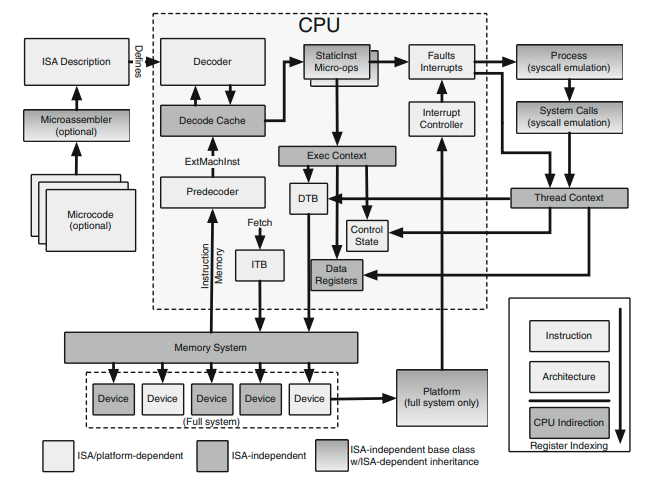
\includegraphics[width=8.5cm]{figs/impl.png}
	\caption{ISA dependency of CPU components}
	\label{fig:isa_dependence}
\end{figure}

To implement the AVR architecture in gem5, we need to implement the following major components:
\begin{itemize}
	\item \textbf{Instruction Set Architecture (ISA)}: The ISA defines the instruction set of the architecture, including:
	      \begin{itemize}
		      \item Arithmetic Logic Unit (ALU) operations (ADD, SUB, AND, OR, etc.)
		      \item Data transfer instructions (MOV, LD, ST)
		      \item Control flow instructions (RJMP, RCALL, RET)
		      \item Bit manipulation instructions (BSET, BCLR, BST, BLD)
	      \end{itemize}

	\item \textbf{Processor Core}: The processor implementation requires:
	      \begin{itemize}
		      \item 32 general-purpose 8-bit registers (R0-R31)
		      \item Program Counter (PC) and Stack Pointer (SP) implementation
		      \item Pipeline stages (fetch, decode, execute, memory, write-back)
		      \item Status Register (SREG) for flags (Zero, Carry, Overflow, etc.)
	      \end{itemize}

	\item \textbf{Memory System}: The AVR memory architecture includes:
	      \begin{itemize}
		      \item Harvard architecture with separate address spaces for program and data
		      \item Three-level memory hierarchy (registers, SRAM, and flash memory)
		      \item Memory-mapped I/O for peripheral access
		      \item EEPROM emulation for non-volatile storage
	      \end{itemize}

	\item \textbf{Peripherals}: Essential peripherals to implement:
	      \begin{itemize}
		      \item Timers/Counters (8-bit and 16-bit)
		      \item Analog-to-Digital Converter (ADC)
		      \item Universal Synchronous / Asynchronous Receiver / Transmitter (USART)
		      \item Interrupt controller for handling 35+ interrupt vectors
	      \end{itemize}
\end{itemize}

We have currently implemented the \texttt{add} and \texttt{sub} instructions. We start by defining \texttt{AVR} class derived from \texttt{SimObjects} class. To implement the instructions, we have to follow the DSL of gem5. The flow of the implementation is as follows:
\begin{figure}[h]
	\centering
	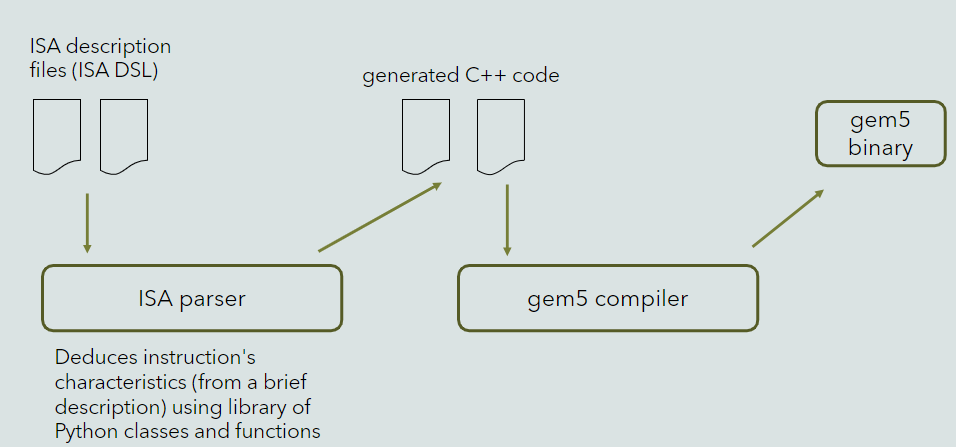
\includegraphics[width=8.5cm]{figs/flow.png}
	\caption{ISA implementation flow}
	\label{fig:implementation_flow}
\end{figure}

The build system of gem5 is based on SCons. The SCons build system is a software construction tool that uses Python scripts to define the build process. The SCons build system is used to build the gem5 simulator and its components. The SCons build system is used to generate the ISA decoder and the instruction set architecture.
\begin{lstlisting}[language=python, caption={Build script in SCons}, label={lst:scons}]
    # -*- mode:python -*-

    Import('*')
    
    DebugFlag('AVR')
    DebugFlag('AVRInst')
    DebugFlag('AVRDecoder')
    
    Source('utility.cc')
    Source('registers.cc')
    Source('faults.cc')
    Source('isa.cc')
    
    
    SimObject('AVR.py', sim_objects=['AVR'])
    
    # Generate ISA decoder
    isa_desc = ISADesc('isa/main.isa')    
\end{lstlisting}
Listing~\ref{lst:scons} shows the SCons build script for the AVR architecture. AVR features are defined across multiple \texttt{.cc} and \texttt{.hh} files. The \texttt{AVR.py} file is the main entry point for the AVR architecture. The \texttt{isa/main.isa} file contains the instruction set description for the AVR architecture. The \texttt{ISADesc} class is used to generate the ISA decoder and the instruction set architecture. The \texttt{DebugFlag} function is used to enable debugging for the AVR architecture.

Going through the implementation of the \texttt{add} instruction, we start by defining the instruction in the \texttt{isa/main.isa} file. It contains the \texttt{bitfield} definition of the instruction. The bitfield definition is used to decode the instruction.

\begin{lstlisting}[language=python, caption={Bitfield definition of the instruction}, label={lst:bitfield}]
def bitfield OPCODE    <15:10>;
def bitfield REG_D     <8:4>;
def bitfield REG_R     <3:0>;
def bitfield IMM8      <7:0>;
\end{lstlisting}

Later operands are defined in the \texttt{isa/operands.isa} file. The operands are used to define the operands of the instruction. The format of \texttt{add} instruction is as follows:
\begin{lstlisting}[language=python, caption={Operands of the instruction}, label={lst:operands}]
def format Add(code, *opt_args) {{
    iop = InstObjParams(name, Name, 'AddOp',
                        {'code': code,
                        'predicate_test': predicateTest,
                        'op_class': 'gem5::enums::IntAlu'
                        },
                        opt_args)
    header_output = AddDeclare.subst(iop)
    decoder_output = AddConstructor.subst(iop)
    decode_block = AddDecode.subst(iop)
    exec_output = AddExecute.subst(iop)
    disasm_output = AddDisassembly.subst(iop)
}};

def template AddDeclare {{
    class %(class_name)s : public gem5::AVRISAInst::AVRStaticInst
    {
      public:
        %(class_name)s(gem5::AVRISAInst::MachInst machInst);
        Fault execute(ExecContext *, trace::InstRecord *) const override;
        std::string generateDisassembly(Addr pc,
            const loader::SymbolTable *symtab) const override;
        void advancePC(PCStateBase &pc_state) const;
    };
}};

\end{lstlisting}
This format is later used by build system to generate the instruction decoder. The functions declared in the \texttt{Add} class is defined later as:
\begin{lstlisting}[language=python, caption={Instruction decoder}, label={lst:decoder}]
def template AddConstructor {{
    %(class_name)s::%(class_name)s(gem5::AVRISAInst::MachInst machInst)
        : gem5::AVRISAInst::AVRStaticInst("add", machInst, %(op_class)s)
    {
        _numSrcRegs = 0;
        _numDestRegs = 0;

        // Source registers: Rd and Rr
        setSrcRegIdx(_numSrcRegs++,
            RegId(gem5::AVRISAInst::intRegClass, bits(machInst, 8, 4)));  // Rd
        setSrcRegIdx(_numSrcRegs++,
            RegId(gem5::AVRISAInst::intRegClass, bits(machInst, 3, 0)));  // Rr

        // Destination register: Rd
        setDestRegIdx(_numDestRegs++,
            RegId(gem5::AVRISAInst::intRegClass, bits(machInst, 8, 4)));

        // Set flags
        flags[IsInteger] = true;
    }

    void %(class_name)s::advancePC(PCStateBase &pc_state) const{
        auto &avr_pc = pc_state.as<gem5::AVRISAInst::PCState>();
        avr_pc.advance();
    }
    std::string
    %(class_name)s::generateDisassembly(Addr pc,
        const gem5::loader::SymbolTable *symtab) const
    {
        std::stringstream ss;
        ss << "add r" << (int)bits(machInst, 8, 4)
            << ", r" << (int)bits(machInst, 3, 0);
        return ss.str();
    }
}};

def template AddExecute {{
    Fault
    %(class_name)s::execute(ExecContext *xc, trace::InstRecord *traceData) const
    {
        // Read source registers
        uint8_t rd = xc->getRegOperand(this, srcRegIdx(0));  // Changed to getRegOperand
        uint8_t rr = xc->getRegOperand(this, srcRegIdx(1));  // Changed to getRegOperand
        uint8_t result = rd + rr;

        // Read SREG
        uint8_t sreg = xc->readMiscRegOperand(this, AVRISAInst::MISCREG_SREG);

        // Update flags
        AVRISAInst::updateFlagsAdd(sreg, result, rd, rr);

        // Write results
        xc->setRegOperand(this, destRegIdx(0), result);  // Changed to setRegOperand
        xc->setMiscRegOperand(this, AVRISAInst::MISCREG_SREG, sreg);

        auto pc = xc->pcState().as<gem5::AVRISAInst::PCState>();
        pc.advance();
        xc->pcState(pc);

        return NoFault;
    }
}};

def template AddDisassembly {{
    std::string
    %(class_name)s::generateDisassembly(Addr pc,
        const gem5::loader::SymbolTable *symtab) const
    {
        std::stringstream ss;
        ss << "add r" << (int)bits(machInst, 8, 4)
            << ", r" << (int)bits(machInst, 3, 0);
        return ss.str();
    }
}};

\end{lstlisting}

The code is later compiled with the SCons build system. To run the simulation, we need to implement the \texttt{AVR CPU} class. The implementation of the \texttt{AVR CPU} is still pending.

\section{Results}
The collected results give us an insight of the effect of different ISAs and \textbf{Cache} models
on performance of code execution.
\subsection{Execution Performance}
The task done by all the ISAs in consideration is same. But the way the C code is translated to
executable instruction is different in different ISAs leading different number of instructions needed to be
performed to do the same amount of job. The \texttt{simInsts} parameters from results report the number 
of simulated instructions.
\begin{figure}[h]
    \centering
    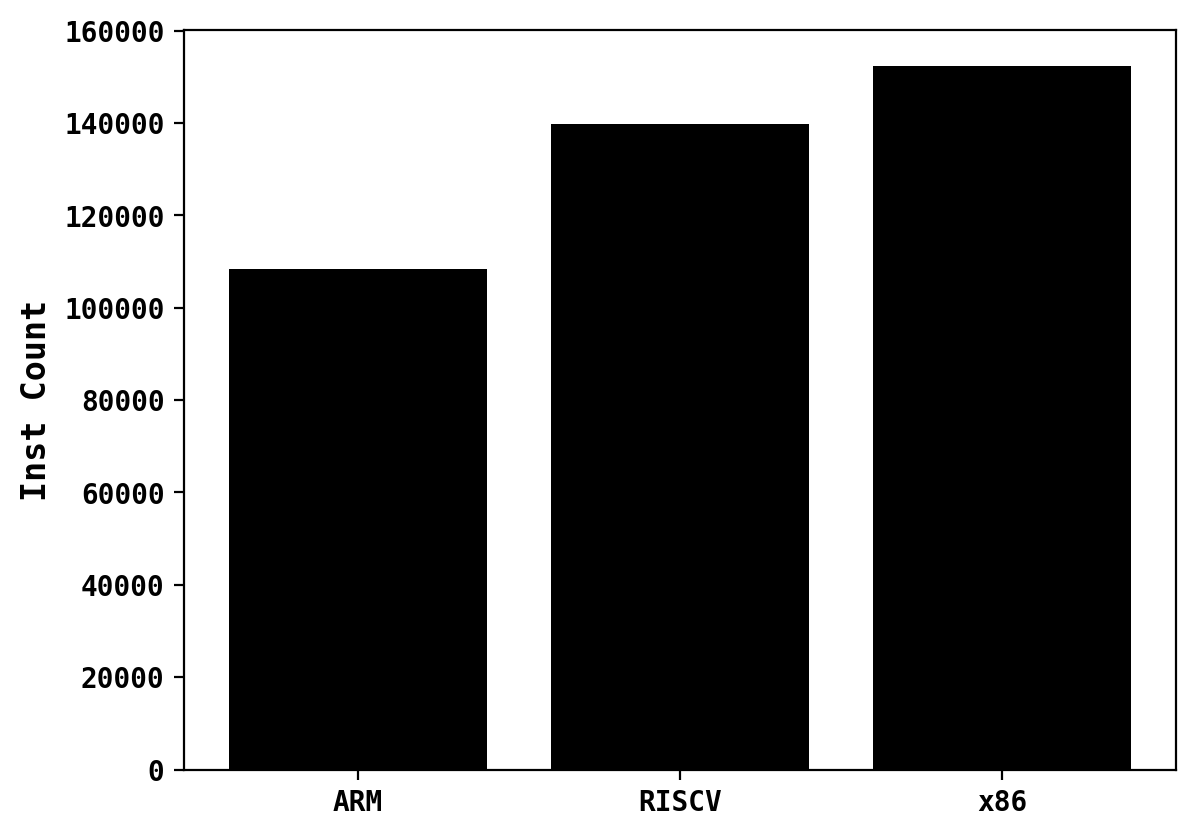
\includegraphics[width=0.8\textwidth]{./figs/1.png}
    \caption{Number of instructions executed by different architectures}
    \label{fig:Number of instructions executed by different architectures}
\end{figure}\\
From the Figure 1, we can note that \texttt{ARM} has to execute minimum number of instructions followed
by \texttt{RISCV} and \texttt{x86}. The simulation was running on a CPU with a clock frequency of
\texttt{1GHz}, implying keeping other parameters constant \texttt{ARM} will perform tasks faster compared to
the other two. This observation can be accounted to the simplicity of the instructions in \texttt{ARM}.
Unlike \texttt{x86}, \texttt{ARM} has fixed length and less number of instructions and a high code density.
Also \texttt{ARM} instructions are highly orthogonal, meaning that most instructions can work with 
any register and support various addressing modes. This reduces the need for special-purpose instructions 
and makes general-purpose ones more versatile. Although \texttt{ARM} and \texttt{RISCV} are based on same 
\texttt{RISC} principle various added advantages like conditional execution and dense addressing modes
allow for lesser instructions than \texttt{RISCV} too.\\
The trend also follows for the number of opcodes and micro-opcodes executed (\texttt{simOps}) during simulation.
\begin{figure}[h]
    \centering
    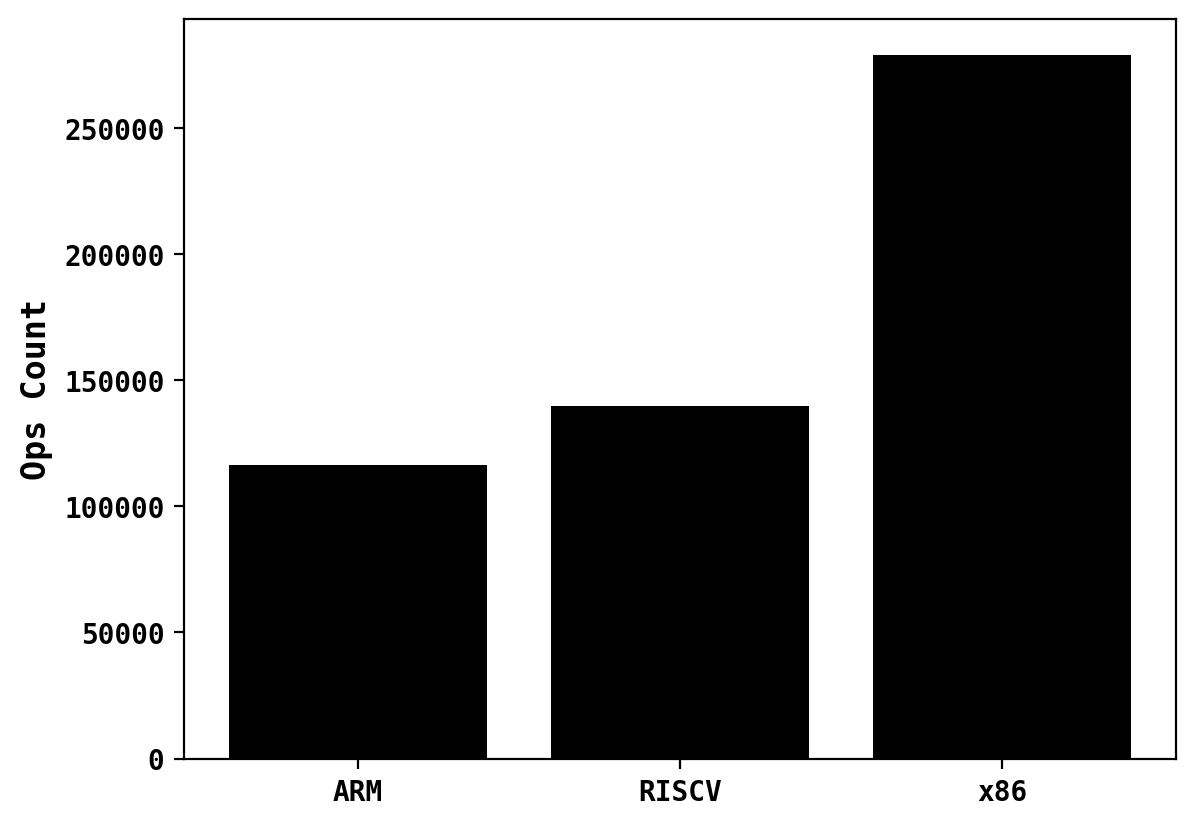
\includegraphics[width=0.8\textwidth]{./figs/2.png}
    \caption{Number of opcodes executed by different architectures}
    \label{fig:Number of opcodes executed by different architectures}
\end{figure}\\
The difference between the number of opcodes executed between \texttt{RISC} based architectures and \texttt{x86}
is stark. \texttt{x86} has to execute roughly 2.3 times more opcodes than \texttt{ARM}. Although \texttt{RISCV} is closer
to \texttt{ARM} with only 1.2 times more opcodes, highlighting the efficiency of \texttt{RISC} based programs.\\
This further translates into the runtime of the programs. From Figure 3, we can say that \texttt{ARM} perform
the task faster with a huge margin compared to others. Specifically, \texttt{ARM} took 1.8 times lesser time
to run than \texttt{x86} and 1.6 times less time than \texttt{RISCV}. Despite having a lower number of instructions
and opcodes the time of execution of \texttt{RISCV} is closer to \texttt{ARM} than \texttt{x86}. This can
be counter-intuitive to think of. But next parameter that we looked on explains this result.\\
As an instruction need not to take only one cycle to execute. In fact most
\begin{figure}[H]
    \centering
    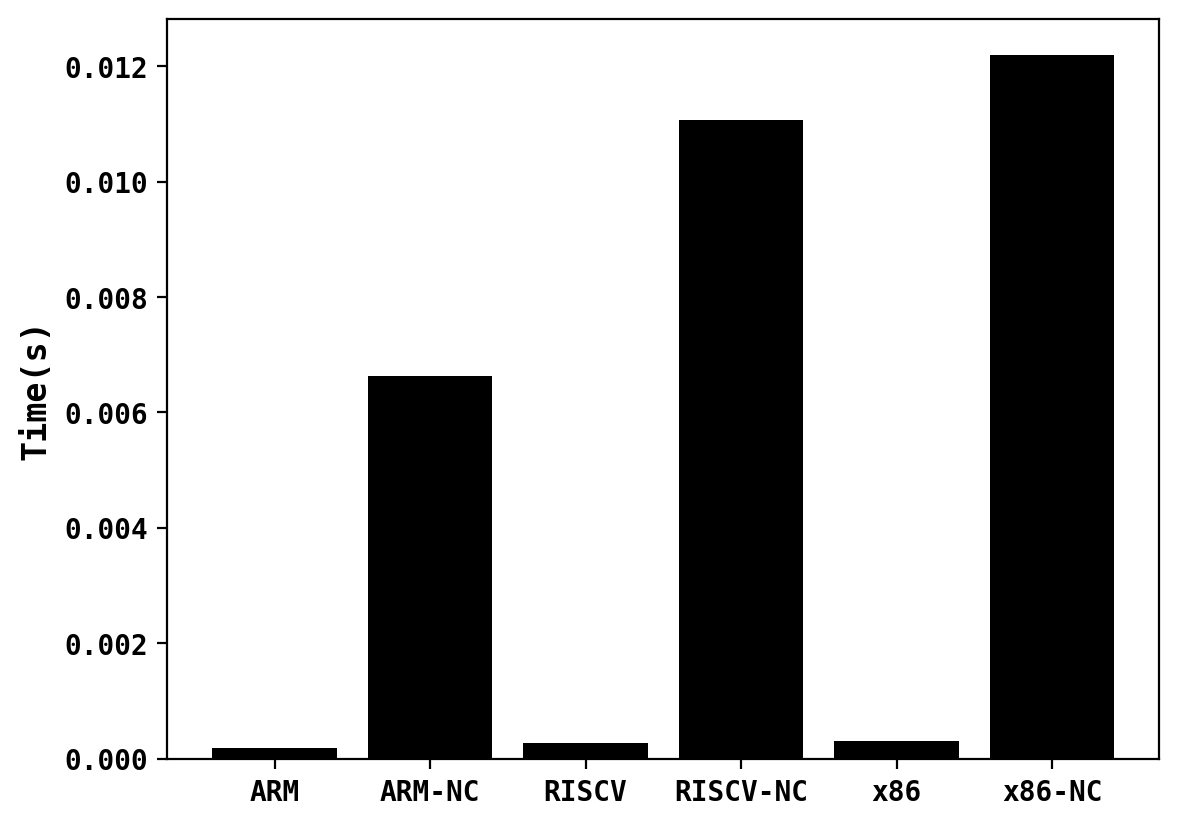
\includegraphics[width=0.8\textwidth]{./figs/3.png}
    \caption{Total execution time}
    \label{fig:Total execution time}
\end{figure}
\begin{figure}[H]
    \centering
    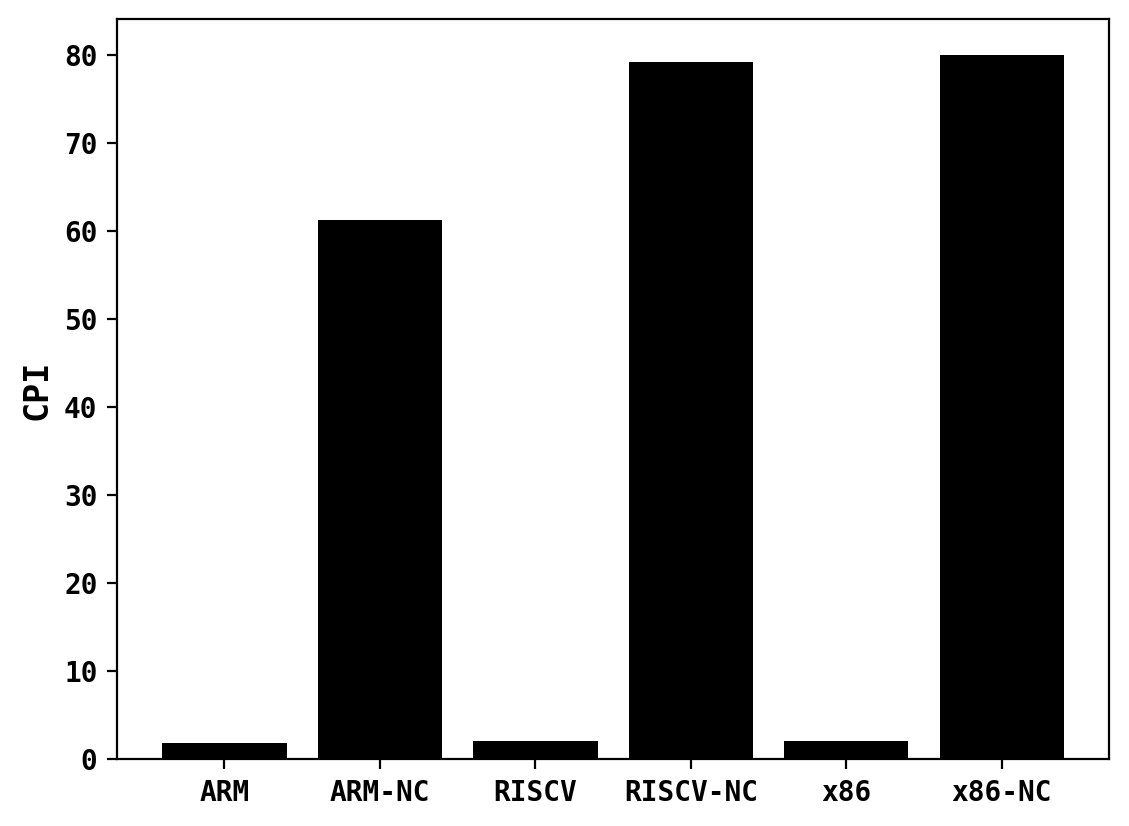
\includegraphics[width=0.8\textwidth]{./figs/4.png}
    \caption{CPI}
    \label{fig:CPI}
\end{figure}
of the instructions take multiple cycles to run. This is measured in \texttt{CPI} or cycles per 
instruction. Figure 4, shows the \texttt{CPI} of different architectures. It's evident that \texttt{RISCV}
uses more cycles to execute a single instruction compared to \texttt{ARM}. It roughly has similar \texttt{CPI}
to \texttt{x86}. Thus, \texttt{RISCV} has a larger execution time than \texttt{ARM}.\\
Overall, \texttt{ARM} performed operations faster as compared to other two mentioned accounting for lower instructions,
opcodes and a lower \texttt{CPI}. 

\subsection{Cache Performance}
\texttt{Cache} works a great deal to improve the performance of the CPU by reducing the bottle-neck of
a slower data transfer rate of the main memory. From Figure 3, the difference between the speed of \texttt{Cache}
versus \texttt{No\_Cache} system is evident. Even the fastest \texttt{ARM} without \texttt{Cache} is much slower than 
\texttt{x86} equipped with \texttt{Cache}. Taking the example of \texttt{ARM}, the \texttt{Cache} version
is roughly 35 times faster than the \texttt{No\_Cache} version of \texttt{ARM} and even \texttt{Cache} version of \texttt{x86}
is roughly 21 times faster than \texttt{No\_Cache} version of \texttt{ARM}. All other \texttt{ISAs} represent a similar
story.
\begin{figure}[H]
    \centering
    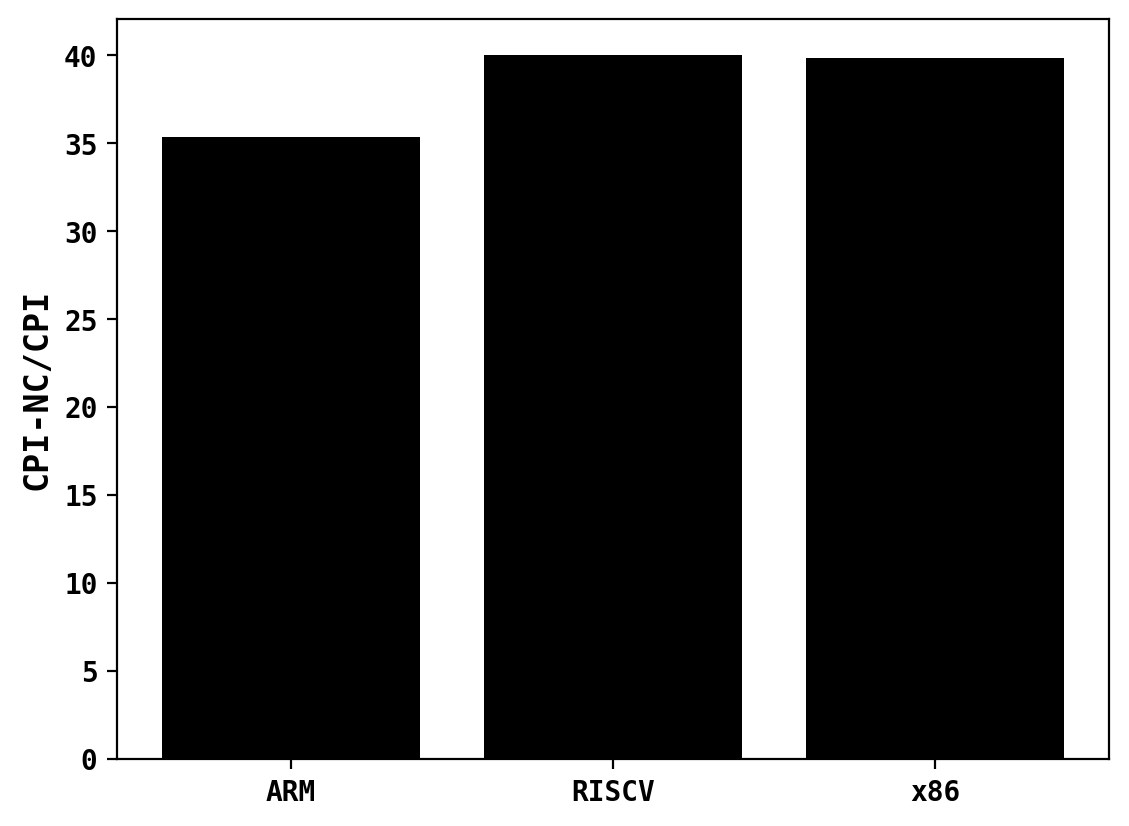
\includegraphics[width=0.8\textwidth]{./figs/5.png}
    \caption{Boost in CPI with addition of \texttt{Cache}}
    \label{fig:Boost in CPI with addition of \texttt{Cache}}
\end{figure}
From Figure 5, the addition of \texttt{Cache} has improved the \texttt{CPI} by a factor of at least 30-35.
All the previous results discussed, were done by keeping the size of problem i.e, size of sieve constant at
100. This is relatively a small problem size. To check the effect of \texttt{Cache} we can increase the problem size.
\begin{figure}[H]
    \centering
    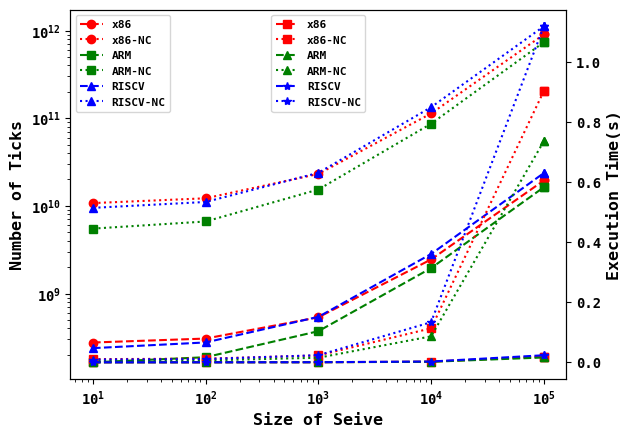
\includegraphics[width=1.0\textwidth]{./figs/6.png}
    \caption{Number of \texttt{Ticks} and execution time w.r.t size of sieve}
    \label{fig:Number of \texttt{Ticks} and execution time w.r.t size of sieve}
\end{figure}
Figure 6 shows some obvious trends that we have discussed earlier, like \texttt{No\_Cache} version are 
slower by large factor and \texttt{ARM} performs better in both \texttt{Cache} and \texttt{No\_Cache} versions
as compared to others. But new interesting observation is that \texttt{RISCV} fares slower than \texttt{x86}
for larger sizes of problem. The gap at the 1e5 between execution time of \texttt{RISCV} and \texttt{x86}
is huge.\\


The cache miss ratio is a crucial parameter in understanding the performance. Figure 7-9 show the cache miss
ratio of various \texttt{cache\_hierarchy}.
\begin{figure}[H]
    \centering
    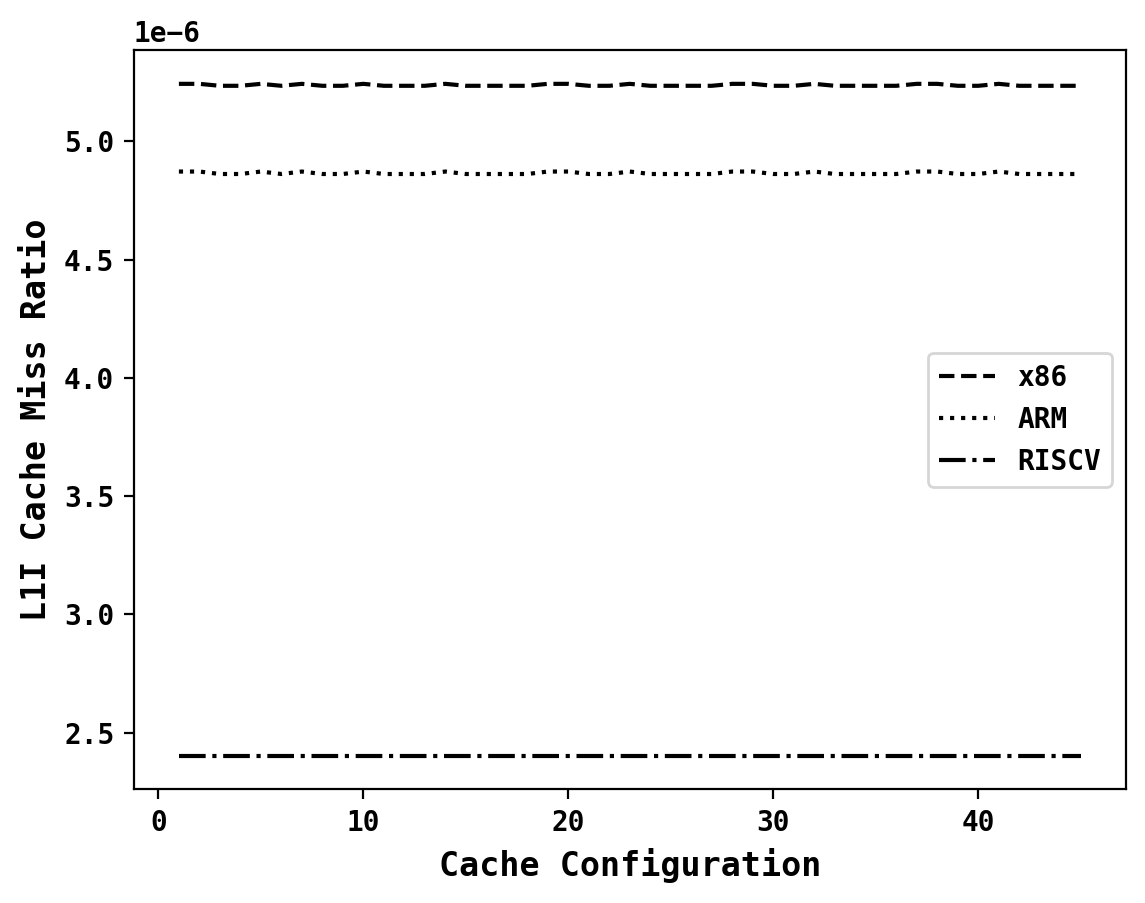
\includegraphics[width=0.8\textwidth]{./figs/8.png}
    \caption{Cache Miss ratio on L1 Instruction Cache}
    \label{fig:Cache Miss ratio on L1 Instruction Cache}
\end{figure}
\begin{figure}[H]
    \centering
    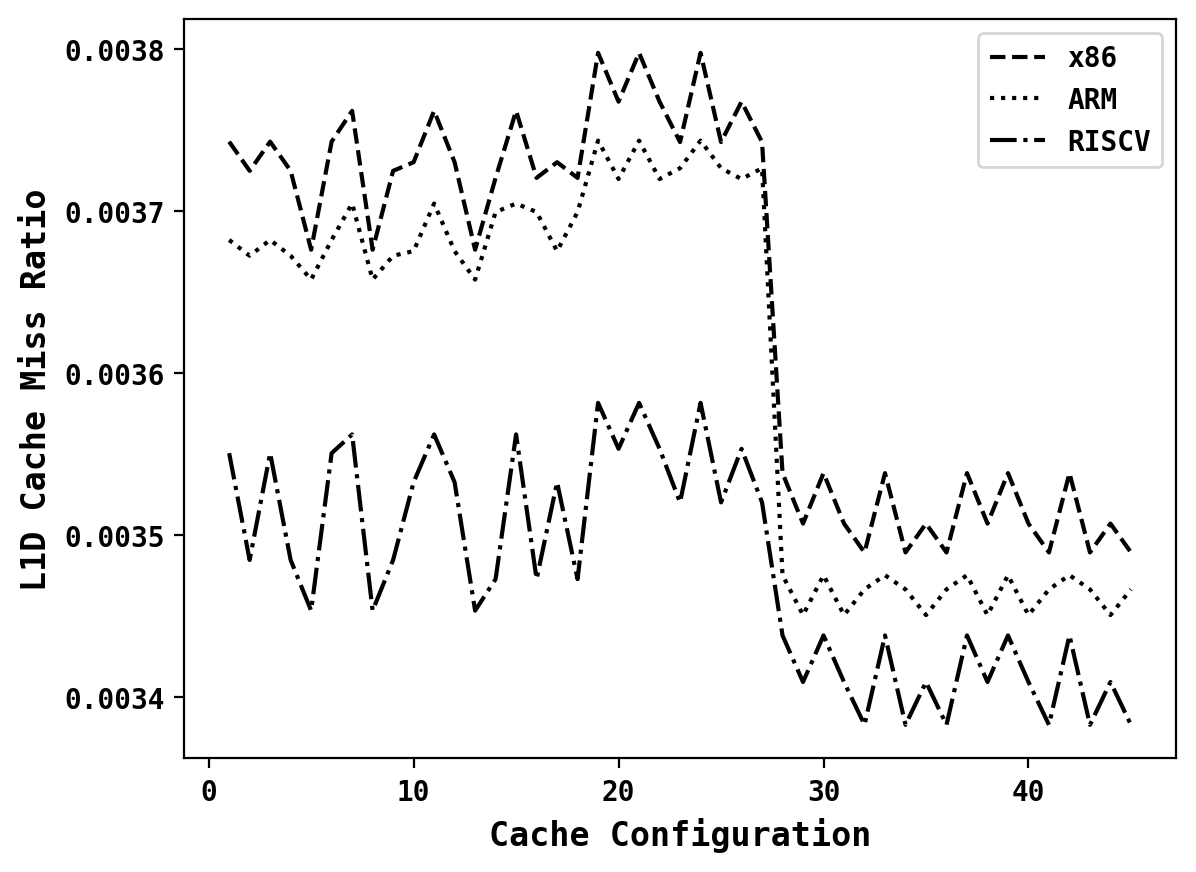
\includegraphics[width=0.8\textwidth]{./figs/7.png}
    \caption{Cache Miss ratio on L1 Data Cache}
    \label{fig:Cache Miss ratio on L1 Data Cache}
\end{figure}
\begin{figure}[H]
    \centering
    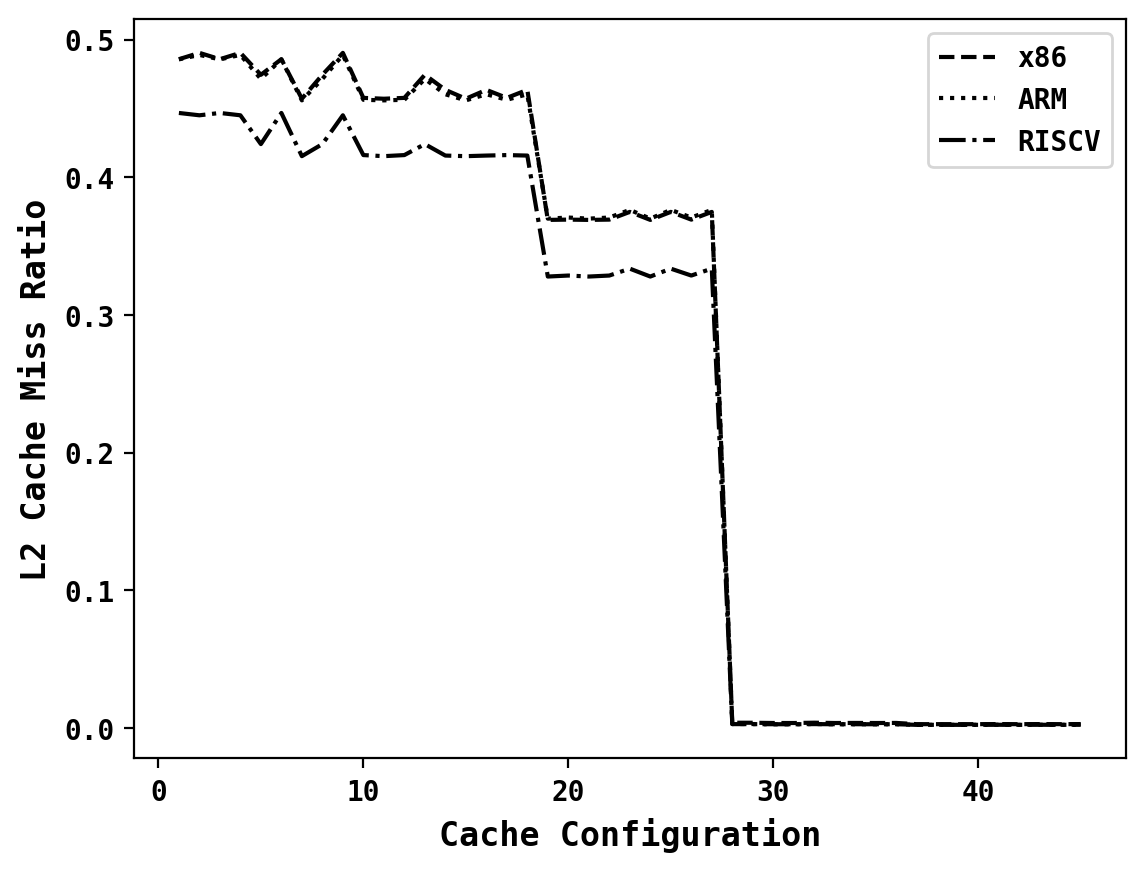
\includegraphics[width=0.8\textwidth]{./figs/9.png}
    \caption{Cache Miss ratio on L2 Cache}
    \label{fig:Cache Miss ratio on L2 Cache}
\end{figure}
From Table 2, there are three parameters affecting the \texttt{cache\_hierarchy},
namely \texttt{L1DSize}, \texttt{L1ISize} and \texttt{L2Size}. Taking the possible value from Table 2 for
each parameters we get a total of 45 configurations. The array all these configurations tuples, is then sorted
taking the sum of total cache as key. The index of these configurations in the sorted array is used to plot
the corresponding results in figures 7-9. For smaller cache sizes \texttt{ARM} and \texttt{x86} tend to perform
similar while \texttt{RISCV} performs best. This trend continues for the \texttt{L1D} cache for larger
cache sizes as well. But for \texttt{L2} cache all the architectures perform similar for larger cache sizes.\\
Figure 6 shows the cache miss ratio of the \texttt{L1I} Cache, across the architectures. Since, total number of
instructions were pretty small a larger cache size doesn't affect the miss ratio. On the other hand from Figure
8 and 9 the increase in cache size leads to significant drop in miss ratio. Specifically in case of the \texttt{L2}
cache the miss ratio drops to 0 for large cache memory. In case of the \texttt{L1D} cache the increase in
size although drops the miss ratio but that is not much significant. Major impact of the size of the cache
is seen on the \texttt{L2}'s miss ratio. Although, the effect can be attributed to the huge size increment
to \texttt{L2} from a mere \texttt{128kB} to \texttt{2048kB}. Nonetheless, all architectures perform close on
the cache miss ratio. The major factor affecting it is size not the architecture itself.

\section{Conclusion}
From the study above, it can be concluded that in light of a simple algorithm of \textbf{Sieve of Eratosthenes}
\texttt{ARM} performs best among the three in terms of speed. It can be credited to the simple yet 
dense instructions of \texttt{ARM}. Also \texttt{RISCV} being from the same \texttt{RISC} family as \texttt{ARM}
performs closer to \texttt{x86}. The cache memory however plays a very significant role in improving
the execution time but it does so for all the ISAs alike. The cache miss ratio discussed is affected most
by the size of the cache than ISA. However, different ISAs produce different cache miss ratio but the 
difference is not significant enough to favour one over other.  

\bibliographystyle{IEEEtran}
\bibliography{references}

\end{document}
